% - Multi-object tracking problem, assumptions
%     - Recall some part from Intro, gradually from JPDA to PHD
% - Object birth/survival

In this section, we provide the theoretical background of the multi-target tracking problem. We have already established the foundations of Bayesian filtering and explained in detail how the Kalman filter works. Now, we will discuss how it differs from other filters that are used for tracking objects. Before we start building the theoretical foundations for object tracking filters, we need to clarify the difference between Bayesian filtering and Bayesian object tracking.

When we track objects, we rely on measurements from sensors, such as cameras, lidars, or radars. These sensors have specific technical specifications and limitations, and there is no sensor that can be 100\% reliable. The reliability of a sensor may be affected by noise, which occurs when a sensor detects an object that is not present. This behavior may be caused by weather conditions in the sensor's operating area, the sensor's limited resolution, or dirt or dust covering the sensor's surface. We do not address the exact reasons why this happens; we only need to find ways to eliminate noisy measurements and separate them from measurements generated by existing objects.

The second problem is closely related to the first. It occurs when a sensor fails to generate measurements for objects that are present in its field of view. The reasons for this may be the same as for noisy measurements, and we do not address these reasons directly. However, we must be able to mathematically model these situations to ensure that they can be properly handled by the filter we want to use to track objects.

These two problems have their names that we will use in this work. Noisy measurements are called \textit{clutter}, and missing measurements are called \textit{misdetections}. We have already seen that the latter problem can be handled by the Kalman filter by skipping the update step. Clutter, on the other hand, creates a much more challenging problem. Figure \ref{fig:clutter-intro} shows what clutter looks like to the filter. In the left image, we see a track of an object and measurements generated by the sensor, shown in red. Clutter measurements are shown as blue asterisks. We can distinguish between measurements and clutter. However, in the right image, we see how the filter sees the same data points, with all points in the same color. To the filter, all these points look the same, and there is no easy way to distinguish between clutter and real measurements.

\begin{figure}
\centering
\begin{subfigure}[t]{.45\textwidth}
  \centering
  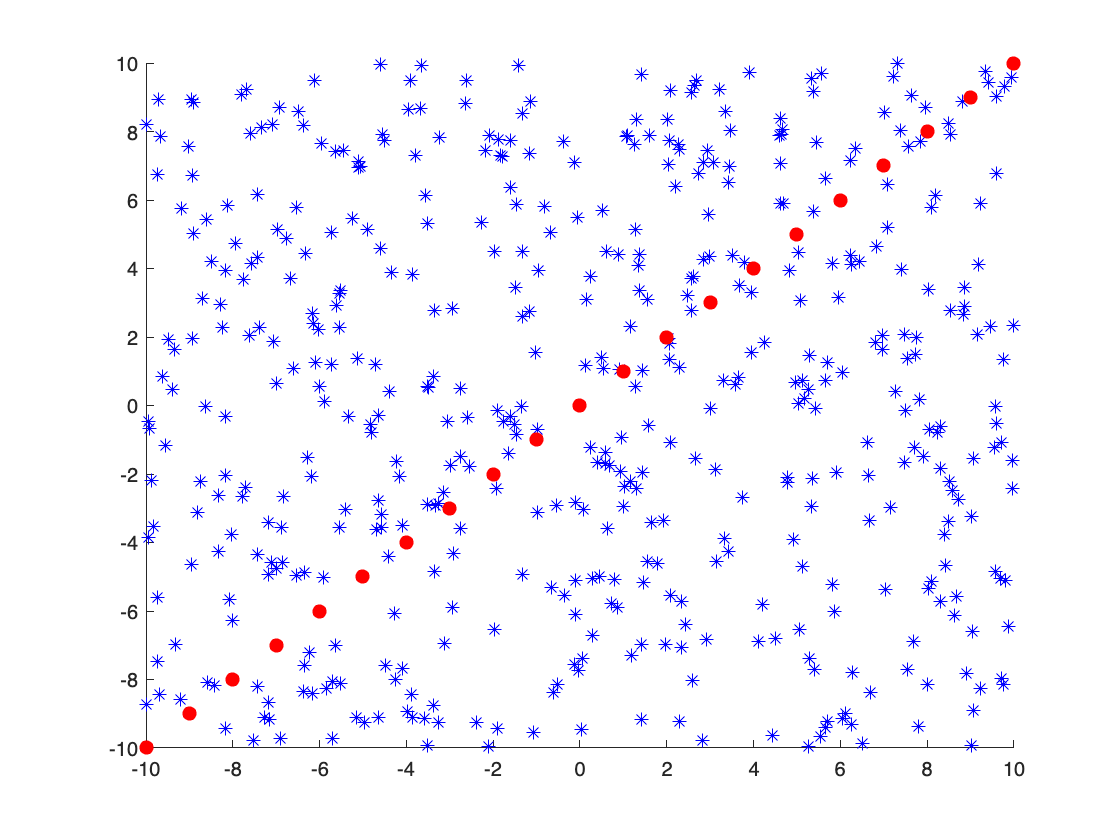
\includegraphics[width=.9\linewidth]{figures/clutter.intro.1.png}
   \caption{Real measurements from some object are shown as red dots. Clutter measurements are displayed as blue asterisks.}
  \label{fig:clutter-intro:1}
\end{subfigure}\hfill
\begin{subfigure}[t]{.45\textwidth}
  \centering
  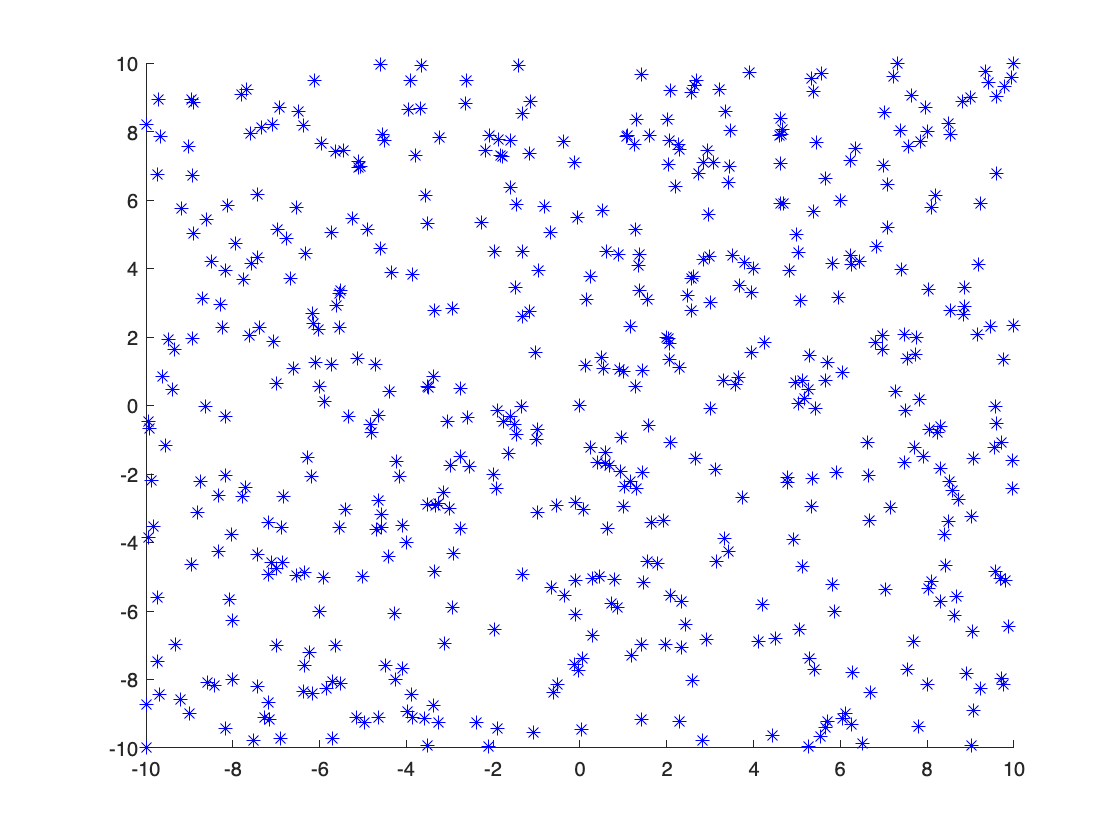
\includegraphics[width=.9\linewidth]{figures/clutter.intro.2.png}
  \caption{Both real measurements and clutter measurements are shown as blue asterisks.}
  \label{fig:clutter-intro:2}
\end{subfigure}
\caption[Measurements in clutter.]{Measurements in clutter. In this Figure, we indicate the clutter problem. When a sensor generates measurements, some of them may be clutter measurements, and there is no easy way to distinguish which data points come from a real object and which are noise.}
\label{fig:clutter-intro}
\end{figure}

The uncertainty in distinguishing between real measurements and clutter has led to the development of many methods for addressing this problem. The main idea behind these methods is that, since we have no information about which measurements come from targets and which are clutter, we should consider all measurements at each time step as coming from a target. This involves creating all possible assignments between measurements and targets and then evaluating the probability of each such assignment. In other words, we evaluate the possibility that a given measurement comes from a specific target according to its motion model. If the measurement is too far from the target, the probability of such an assignment will be lower than that of an assignment with a measurement that is close to the predicted state. These assignments are referred to as \textit{association hypotheses}. In the following subsection, we will provide a brief overview of various target tracking methods and approaches. But before doing so, we will outline the main assumptions of multi-target tracking (MTT).
